\documentclass{standalone}

\usepackage[american]{circuitikz}

\begin{document}
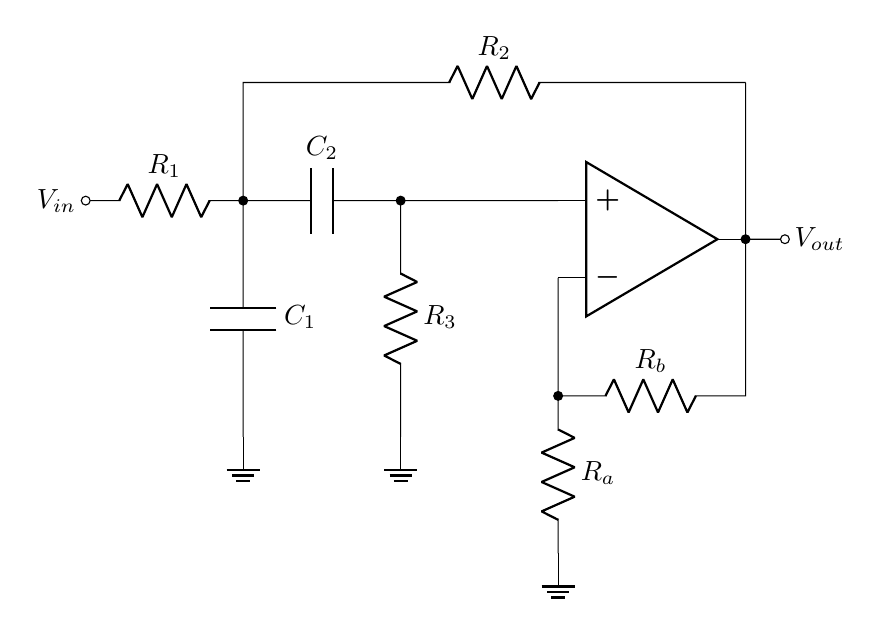
\begin{tikzpicture}[american voltages]
	\draw
	(0,0.5) node[op amp, yscale=-1] (opamp1) {}
	(opamp1.+) to [short, -*] ++(-2,0)
	to [R, l=$R_3$] ++(0, -3)
	to ++(0,0) node[ground] {}
	(opamp1.+) -- ++(-2, 0) 
	to [C, l_=$C_2$, -*] ++(-2,0) coordinate (node1)
	to [C, l=$C_1$] ++(0, -3) node[ground] {}
	(node1) to [R, l_=$R_1$, -o] ++(-2,0) node[left] {$V_{in}$}
	(node1) to [short] ++(0,1.5)
	to [R, l=$R_2$] ++(6.38,0) coordinate(node3)
	(opamp1.-) to [short, -*] ++(0,-1.5) coordinate(node2)
	(node2) to [R, l=$R_b$] ++(2.35,0) -| (opamp1.out)
	(node2) to [R, l=$R_a$] ++(0, -2) node[ground] {}
	(opamp1.out) to [short,  *-] ++(0,0) -| (node3)
	(opamp1.out) to [short, -o] ++(0.5,0) node[right] {$V_{out}$}
	;
\end{tikzpicture}
\end{document}